\chapter{Bush ed Engelbart, Memex e Demo}

\section{Introduzione}

\dfn{Knowledge Navigator}{
    Un'idea di Apple, presentata nel 1987, di un assistente virtuale
    che aiuta l'utente a navigare tra le informazioni.
}

\subsubsection{Il filmato di presentazione del Knowledge Navigator (1987):}

\begin{itemize}
    \item [$\Rightarrow$] \fancyglitter{La comprensione del parlato}:
    il computer capisce il linguaggio naturale;
    \item [$\Rightarrow$] \fancyglitter{La grafica e le finestre}:
    dietro questo video c'è Alan Kay, che ha lavorato a Xerox PARC e fu 
    l'inventore delle finestre;
    \item [$\Rightarrow$] \fancyglitter{Il touch screen};
    \item [$\Rightarrow$] \fancyglitter{La videochiamata};
    \item [$\Rightarrow$] \fancyglitter{La simulazione}: della desertificazione.
\end{itemize}

\qs{}{Chi era Vannevar Bush?}

\paragraph{Risposta:} Vannevar Bush (1890 - 1974) era un ingegnere e scienziato americano.
Lui teorizzò il Memex
(non fu mai realizzato).

\nt{Durante una conferenza in occasione del 50° anniversario di "As 
we may think" (1945) venne presentata un'animazione del Memex.}

\section{Il Memex}

\dfn{Memex}{
    Un sistema di archiviazione e ricerca delle informazioni, teorizzato da Vannevar Bush.
}

\nt{Il Memex offre anche un'anticipazione di ciò che sarà l'\fancyglitter{
    ipertesto}, che nascerà vent'anni dopo.
}

\subsection{Problemi di organizzazione dell'informazione}

Il problema che preocupa Bush è \fancyglitter{la perdita di informazioni} che si accumula
continuamente nel tempo\footnote{Questo problema non era nuovo. 
Era già stato affrontato da Paul Otlet.}. Inoltre si aumenta progressivamente la
specializzazione: le informazioni sono sempre più frammentate e sempre più
specializzate (più difficili da comunicare). Bush ritiene che il problema 
non sia l'eccesso di pubblicazioni, ma il fatto che si siano estese oltre
la capacità di gestione dei documenti. 
La \fancyglitter{selezione}\footnote{Processo di scelta delle informazioni.}
è un problema per via delle enormi quantità di informazioni.

\ex{Addetto dell'ufficio informazioni}{
    L’addetto all’ufficio del personale di una fabbrica immette una pila di alcune migliaia di schede
degli impiegati in una macchina selezionatrice, imposta un codice secondo una convenzione
stabilita e produce in poco tempo una lista di tutti gli impiegati che vivono a Trenton e
conoscono lo spagnolo.
}

\ex{Centralini telefonici automatici}{
    Si compone un
numero e la macchina seleziona e connette solamente una tra un milione di possibili stazioni.
Non le ispeziona tutte. Presta attenzione solo a una classe data dalla prima cifra, poi solo a una
sottoclasse data dalla seconda cifra e così via; così procede rapidamente e quasi infallibilmente
verso la stazione selezionata.
}

\paragraph{Prroblemi di indicizzazione:}

\begin{itemize}
    \item [$\Rightarrow$] Si cerca da sottoclasse a sottoclasse;
    \item [$\Rightarrow$] L'informazione si trova in un unico punto (a meno che non sia duplicata);
    \item [$\Rightarrow$] Bisogna avere regole per specificare il percorso, ma le regole sono complicate;
    \item [$\Rightarrow$] Quando si trova l'elemento bisogna riemergere dal sistema e rientrare attraverso un nuovo percorso.
\end{itemize}

\nt{La situazione peggiore, ma più facilmente verificabile, è la ricerca in un albero.}

\dfn{Classificazione}{
    La \newfancyglitter{classificazione} è una segmentazione spaziale, temporale o spazio-temporale del mondo.
    
    Un sistema di classificazione è un insieme di scatole in cui si mettono cose per fare un 
    qualche tipo di lavoro.
}

\paragraph{Proprietà di un sistema di classificazione:}

\begin{itemize}
    \item [$\Rightarrow$] Ci sono principi univoci e consistenti;
    \item [$\Rightarrow$] Le categorie sono reciprocamente esclusive;
    \item [$\Rightarrow$] Il sistema è completo.
\end{itemize}
\pagebreak
\begin{figure}[h]
    \centering
    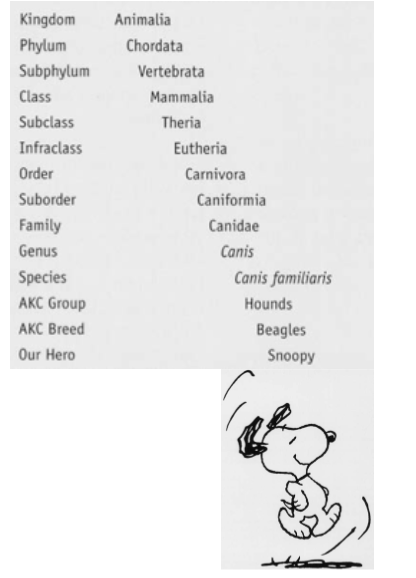
\includegraphics[scale=0.5]{images/Snoopy.png}
    \caption{Snoopy secondo due sistemi di classificazione.}
\end{figure}

\subsection{Indicizzazione}

\dfn{Indicizzazione}{
    L'\newfancyglitter{indicizzazione} è un'operazione è l'azione di descrivere o identificare
    un documento (o un oggetto) nei termini del suo contenuto concettuale\footnote{ISO 5963.}.
}

\nt{Lo scopo generale dell'indicizzazione è quello di rappresentare oggetti
in modo che possano essere efficacemente trovati e utilizzati.}

\cor{Linguaggio di indicizzazione}{
    Un linguaggio di indicizzazione è un sistema di rappresentazioni simboliche (un codice)
    che consentono la classificazione e la ricerca di documenti attraverso
    i codici assegnati ai concetti che essi contengono (indicizzazione per concetti).
}

\nt{Ted Nelson, in "As we may think", criticherà il fraintendimento
per cui si vede nel lavoro di Bush un contributo alla information retrieval\footnote{Reperimento di oggetti informativi.}.
}


\subsection{Browser vs Search}

Le seguenti definizioni sono state date da Clay Shirky in "Ontology is Overrated. 
Categories, Links, and Tags" (2005).

\dfn{Browse}{
    \newfancyglitter{Browse} significa che le persone fanno ontologia
    e categorizzazione, avendo la responsabilità di organizzare il mondo in anticipo.
}

\nt{Il browse è uno schema passivo.}

\dfn{Ricerca}{
    Il paradigma della \newfancyglitter{ricerca} sostiene che nessuno può
    prevedere cosa sarà necessario in futuro. Quando se ne ha bisogno si tenterà
    di trovarlo basandosi sulla struttura di link disponibile.
}

\nt{Per esempio, Google è un sistema di ricerca.}

\subsection{Associazione}

La mente umana, secondo Bush, lavora per associazione: quando 
"afferra" un elemento scatta istantanemente a quello successivo in base 
a un'associazione di pensieri in accordo con una rete di percorsi determinata dai neuroni.
La selezione per associazione può essere meccanizzata dal \fancyglitter{Memex}.

Nel Memex vengono archiviati tutti i libri, le registrazioni e le comunicazioni.
Esso è meccanizzato in modo da essere consultato con estrema velocità e flessibilità.
Si tratta di un supplemento \fancyglitter{personalizzato} ed allargato alla memoria dell'individuo.

\paragraph{Il Memex è uno strumento \textit{personale}:}

\begin{itemize}
    \item [$\Rightarrow$] È utilizzato da una sola persona;
    \item [$\Rightarrow$] L'utilizzatore lo adatta ai propri interessi;
    \item [$\Rightarrow$] Il Memex non è collegato ad altri dispositivi (non esiste una rete di Memex).
\end{itemize}

\nt{Il Memex è stato disegnato da Alfred D. Crimi, in Life.}

\clm{}{}{
    La versione del Memex su Life è stata letta da Engelbart in una 
    baracca della croce rossa nelle Filippine. Engelbart rievocherà
    questa descrizione tra la fine degli anni '50 e l'inizio degli anni '60
    quando deciderà di dedicarsi ad alcune problematiche di cui aveva avuto
    un'anticipazione nell'articolo di Bush.
}

\subsection{Le funzionalità del Memex}

La maggior parte dei contenuti del Memex è archiviata su microfilm (con rapid selector).
Il microfilm è un grande limite del Memex, in quanto analogico.

\paragraph{Le potenzialità del collegare elementi:}

\begin{itemize}
    \item [$\Rightarrow$] Fornisce un passo verso un'\fancyglitter{indicizzazione associativa}\footnote{Qualsiasi elemento può immediatamente selezionarne automaticamente un altro};
    \item [$\Rightarrow$] Quando un utente crea un percorso, il Memex lo \fancyglitter{nomina},
    \fancyglitter{inserisce il nome nel libro dei codici} e lo batte sulla tastiera;
    \item [$\Rightarrow$] In fondo a ogni elemento ci sono degli \fancyglitter{spazi vuoti} per immettere dei codici e viene impostato un puntatore per indicarne uno per ciascun elemento;
    \item [$\Rightarrow$] L'utente preme un singolo tasto e gli elementi vengono uniti in modo permanente\footnote{Nei relativi spazi appare il codice.}.
\end{itemize}

\subsubsection*{}
Questo processo fa si che, in qualsiasi momento, quando uno di questi elementi
viene richiamato, venga richiamato anche l'altro\footnote{Proprio come un ipertesto.}.
Si può dire che gli oggetti fisici siano stati raccolti da fonti remote e rilegati
insieme per \fancyglitter{formare un nuovo libro}\footnote{
    Quest'idea (un libro costruito attivamente da chi lo sta consultando), anticipata da Otlet,
    verrà ripresa da Licklider a proposito delle \fancyglitter{biblioteche del futuro}.
}.


\ex{Un Caso d'Uso del Memex}{
    \subsubsection{Questo esempio è ripreso parola per parola dalle slides del prof. Cardone.}

    Poniamo il caso che il proprietario del memex sia interessato all’origine e alle proprietà dell’arco
e delle frecce. Più precisamente egli sta studiando la ragione per cui l’arco corto turco fu
apparentemente migliore dell’arco lungo inglese nei combattimenti delle Crociate.

Egli ha dozzine di libri e articoli potenzialmente pertinenti nel suo memex.

Prima sfoglia un’enciclopedia, trova un articolo interessante ma non abbastanza dettagliato, e lo
lascia proiettato. Poi, in un libro di storia, trova un altro articolo pertinente e collega i due
insieme. Procede in questo modo, creando un percorso composto da molti elementi.

Occasionalmente inserisce un proprio commento, collegandolo al percorso principale o,
attraverso un percorso laterale, a uno specifico elemento.

Quando diventa evidente che le proprietà di elasticità dei materiali a disposizione avevano
molto a che fare con l’arco, egli crea una ramificazione su un percorso laterale che lo porta a testi
sull’elasticità e a tabelle di costanti fisiche.

Egli inserisce una pagina di analisi scritta a mano da lui stesso.

Quindi crea un percorso di suo interesse attraverso il labirinto dei materiali a sua disposizione.
Diversi anni più tardi [c]on un tocco accede al libro dei codici. Premendo alcuni tasti egli proietta
l’inizio del percorso. Con una leva lo scorre a piacere fermandosi sugli elementi interessanti,
facendo delle digressioni.

Appariranno tipi totalmente nuovi di enciclopedie, già munite di una rete di tracce associative
che le attraversano, pronte per essere immesse nel memex dove vengono ampliate. [Esempi
sull’uso di una grande massa di informazioni da parte di avvocati, medici e scienziati.]

Lo storico con un vasto resoconto cronologico di un popolo lo accosta ad un percorso saltuario
che si sofferma solamente sui temi salienti, e può seguire in ogni momento percorsi paralleli che
lo portano a spaccati di civiltà in particolari epoche.

}

\clm{}{}{
    Wikipedia è nata in un'ottica di collegamenti e di ipertesto. 
    Il concetto di \fancyglitter{wiki} è stato inventato da Ward Cunningham. 
    Il wiki è ispirato agli ipertesti e fu implementato per la prima volta in \fancyglitter{HyperCard}.
    Inoltre Cunningham è anche noto in ambito di programmazione OO per l'Extreme Programming (XP), visto nel corso 
    "Sviluppo Applicazioni Software".
}

\dfn{Apripista}{
    Un'\newfancyglitter{apripista} è una nuova professione che si occupa di
    stabilire \newfancyglitter{percorsi utili} attraverso l'enorme massa delle informazioni
    archiviate.
}

\section{Il progetto di Doug Engelbart: Demo}

\begin{itemize}
    \item [$\Rightarrow$] 1945: Legge "As we may think" di Vannevar Bush;
    \item [$\Rightarrow$] 1957: Entra alla Stanford Research Institute (SRI);
    \item [$\Rightarrow$] 1962: Pubblica il rapporto "Augmenting Human Intellect: A Conceptual Framework";
    \item [$\Rightarrow$] 1963: partono i finanziamenti per il progetto allo "Augmentation Research Center" (ARC)
    \footnote{Anche grazie a Licklider.};
    \item [$\Rightarrow$] 1968: La "madre di tutte le dimostrazioni" (Demo), San Francisco;
    \item [$\Rightarrow$] 1969: Primo collegamento ARPANET\footnote{Uno dei primi nodi a essere associati ad ARPANET fu proprio quello del SRI.} (tra UCLA e ARP).
\end{itemize}

\dfn{Augmenting Human Intellect}{
    \newfancyglitter{Augmenting Human Intellect} (il rapporto del 1962) contiene la proposta
    del progetto e \newfancyglitter{anticipa} tutte le realizzazioni tecnologiche fino al 1968.
    Esso punta a migliorare l'efficacia intelettuale dell'uomo, scivolando nell'interazione/simbiosi tra uomo e macchina.
}

\clm{}{}{
    A un certo punto del progetto si fece uso di uno strumento hardware a 5 dita e gli operatori
    comunicavano tra loro, da una postazione all'altra, mostrando le dita della mano.
}

\subsection{L'idea di "Augmentation"}

Engelbart puntava ad affrontare i problemi "\fancyglitter{complessi}": di diplomatici,
di scienziati, di fisici, avvocati, etc.. Questi problemi vanno affrontati 
non tramite trucchetti, ma comprendendo il problema. I problemi possono 
essere ben posti/tame problems o mal posti/wicked problems (sul lato della progettazione\footnote{
    Un esempio è la pianificazione di una linea di metropolitana. I problemi
    urbanistici sono generalmente wicked problems.
}).

\begin{figure}[h]
    \centering
    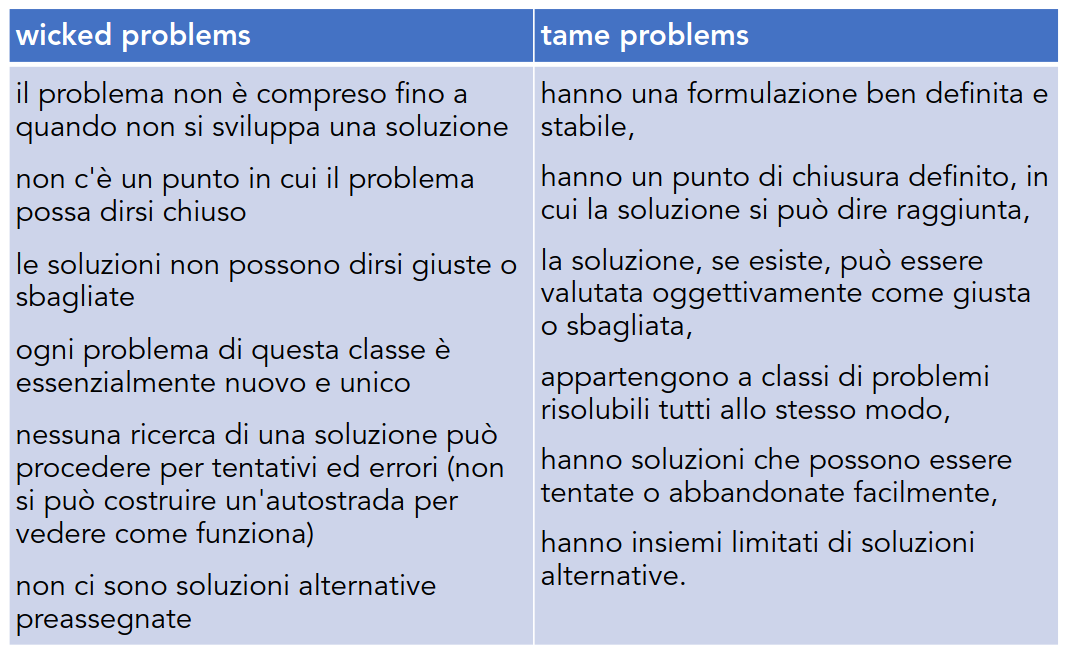
\includegraphics[scale=0.35]{images/Problems.png}
    \caption{Problemi mal posti vs. Problemi ben posti.}
\end{figure}

\nt{La questione dei problemi mal posti e ben posti è affrontata 
approfonditamente nel corso "Metodologie e Tecnologie Didattiche per l'Informatica".}

\ex{Quali wicked e quali tame?}{
    Con \textcolor{red}{\XSolidBrush} si indicano i wicked problems e con \textcolor{green}{\Checkmark} i tame problems.

    \begin{itemize}
        \item [\textcolor{green}{\Checkmark}] Trovare la radice quadrata di 7358;
        \item [\textcolor{green}{\Checkmark}] Trovare il cammino più breve tra un punto A e un punto B;
        \item [\textcolor{red}{\XSolidBrush}] Progettare un'automobile sicura;
        \item [\textcolor{green}{\Checkmark}] Riparare una lavatrice;
        \item [\textcolor{red}{\XSolidBrush}] Costruire una linea di metropolitana.
        \item [\textcolor{green}{\Checkmark}] Racimolare 10.000 euro;
        \item [\textcolor{red}{\XSolidBrush}] Organizzare una mostra;
        \item [\textcolor{red}{\XSolidBrush}] Preparare un disegno di legge.
    \end{itemize}


}

\ex{Un architetto "aumentato"}{
    Engelbart racconta l'esempio di un architetto che sta progettando un edificio.

    \paragraph{Attività di questo architetto aumentato da un computer (il "\fancyglitter{clerk}"):}
    \begin{itemize}
        \item [$\Rightarrow$] Ha già fantasticato su diverse strutture e le \fancyglitter{mette alla prova sullo schermo};
        \item [$\Rightarrow$] Sullo schermo ha una \fancyglitter{vista prospettica} del sito di costruzione sul 
        pendio della collina sormontata dalla sede stradale, rappresentazione dei vari alberi che devono rimanere
        sul terrebìno e i vari punti di allacciamento per i servizi;
        \item [$\Rightarrow$] Con il \fancyglitter{puntatore} indica due punti di interesse;
        \item [$\Rightarrow$] Dopo un po' l'architetto \fancyglitter{cambia la scena} sullo schermo in una visione dall'alto che mostra lo scavo;
        \item [$\Rightarrow$] \fancyglitter{Immette con la tastiera un elenco di elementi} controllandoli uno a uno mentre appaiono sullo schermo, rimandandone lo studio in seguito.
    \end{itemize}


}

\subsection{Classi di Strumenti di Aumentazione}

\begin{itemize}
    \item [$\Rightarrow$] \fancyglitter{Artefatti}: oggetti fisici progettati per la comdità dell'uomo,
    per la manipolazione di cose, materiali e simboli;
    \item [$\Rightarrow$] \fancyglitter{Linguaggio}: i modi in cui l'individuo segmenta l'immagine del 
    mondo in concetti che la sua mente usa per modellare, i simboli che associa a 
    quei concetti e utilizza nella manipolazione conscia dei concetti (il "pensiero");
    \item [$\Rightarrow$] \fancyglitter{Metodologia}: i metodi, le procedure e le strategie con cui un individuo
    organizza la sua attività finalizzata alla soluzione di problemi;
    \item [$\Rightarrow$] \fancyglitter{Addestramento (training)}: il condizionamento necessario all'essere umano per portarlo a utilizzare 
    i precedenti elementi in modo efficace.
\end{itemize}

\clm{}{}{Questo sistema è: Trained Human being
together with his Language, Artefacts and Methodology (H-LAM/T\footnote{"Purtroppo Engelbart usava degli acronimi assurdi",
citazione necessaria del prof. Cardone}).
Un esempio di un sistema H-LAM/T sono delle possibili "biblioteche del futuro" (Licklider) in cui sono presenti vari artefatti (scaffali, schedari, etc.), componente umana 
(bibliotecari, catalogatori, etc.), l'addestramento (dei bibliotecari). Il tutto ciò poteva essere sostituito da loro versioni digitali
che "ri-media" dei media analogici in digitali.}

\clm{}{}{
    Benjamin Lee Whorf, ingegnere chimico e poi linguista, affermava che il linguaggio influenza il pensiero.

    Whorf studiava le lingue dei nativi americani, insieme a Edward Sapir. Questi due linguisti
    formularono l'ipotesi per cui la concettualizzazione del mondo dipendesse dal linguaggio.

    IN "Science and Linguistics" Whorf mostrò il modo di segmentare le esperienze di varie popolazioni
    a confronto con quello degli inglesi. Per esempio il fatto che gli eskimesi avessero diverse parole per "neve".

    Per ricollegarci al tema di questo corso, Whorf influenzo gli informatici come Nelson (che si vedrà più avanti) ed 
    Engelbart (che lo cita direttamente nel suo lavoro).
}

\subsection{Il Memex come strumento per la strutturazione simbolica}

I percorsi associativi del Memex forniscono una capacità di strutturazione di simboli che
deriva da una nuova capacità in termini di artefatti e processi\footnote{Il Memex è un artefatto
che supporta queste nuove strutture di concetti.}. Inoltre il Memex può aumentare le 
capacità umane di strutturazione ed esecuzione dei processi.
Engelbart poneva un altro esempio: un sistema di \evidence{schede a bordi perforati [edge-notched]}, a funzionamento
manuale. Le "registrazioni unitarie", a differenza di quelle del Memex, 
sono pezzi di testo o manoscritti su \fancyglitter{schede di formato IBM a bordi perforati}.
Esse sono dati, pensieri, fatti, considerazioni, concetti, idee, preocupazioni, etc. pertinenti
a un \fancyglitter{determinato problema}. 

\begin{figure}[h]
    \centering
    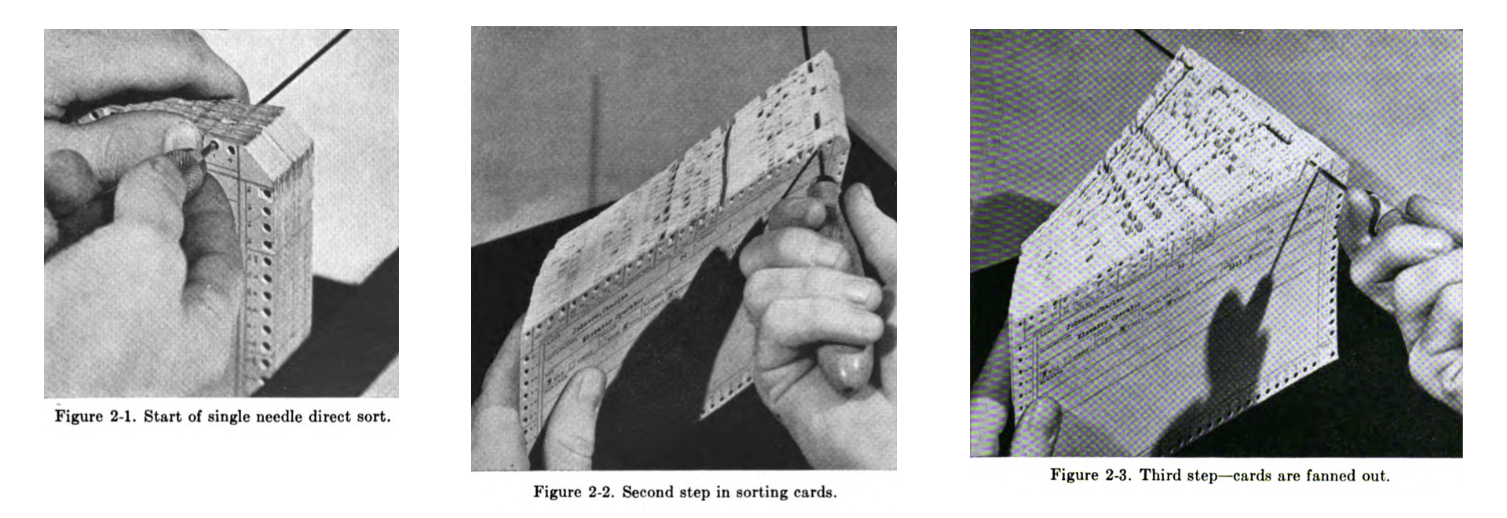
\includegraphics[scale =0.3]{images/Schede.png}
    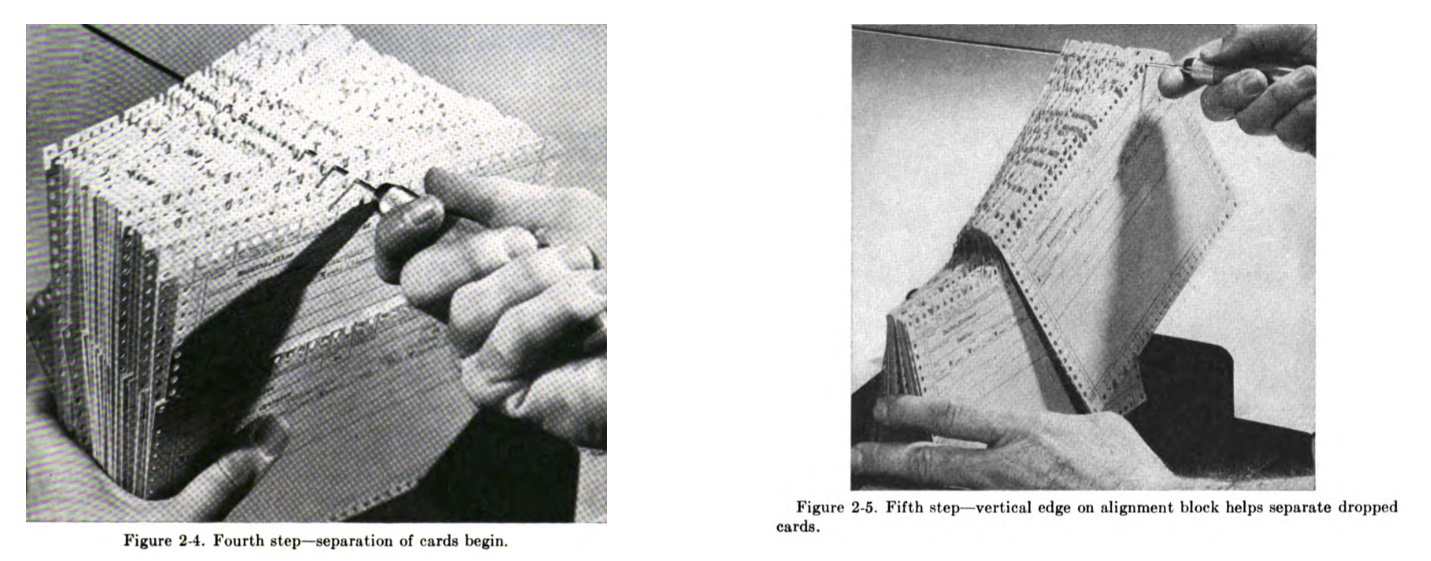
\includegraphics[scale =0.3]{images/Schede2.png}
    \caption{Gestione delle schede perforate.}
\end{figure}

\nt{Queste schede sono alla base di HyperCard, il primo sistema di ipertesto.}

\clm{}{}{
    La novità dell'utilizzo di queste "card" è l'utilizzo di unità minime di
    informazione, di insiemi di argomento ristretto che forniscono grande flessibilità  
    e capacità di manipolazione. Esse mettono a disposizione uno \fancyglitter{spazio di lavoro}
    che si può sfogliare\footnote{"Browse".}, a cui si possono fare aggiunte o correzioni e che
    permettono la costruzione di nuovi insiemi di nuclei di pensieri.
}

\subsection{Utilità del computer}

\begin{itemize}
    \item [$\Rightarrow$] Un computer è direttamente in grado di eseguire processi primitivi di manipolazione simbolica;
    \item [$\Rightarrow$] Con quei processi primitivi si possono costruire ogni altro processo che possa essere descritto da un linguaggio;
    \item [$\Rightarrow$] Un programma è una struttura di processi primitivi memorizzato sotto forma di simboli;
    \item [$\Rightarrow$] I computer hanno vari modi per memorizzzare simboli in modo che possano essere manipolati;
    \item [$\Rightarrow$] È possibile descrivere al computer nuovi simboli;
    \item [$\Rightarrow$] L'interfaccia è il punto di contatto tra l'uomo e la macchina (nascita dell'interazione uomo-macchina\footnote{Importante il time-sharing});
    \item [$\Rightarrow$] 1962: \textit{un programma sperimentale di ricerca che è ancora lontano alcuni anni dalla fase presente della sua realizzazione} (DEMO del 1968).
\end{itemize}

\section{Panoramica della DEMO}

\paragraph{Sezioni:}

\begin{enumerate}
    \item La più celebre introduzione dell'informatica, descrive, in tono epico,
    la situazione che il sistema nLS intende aumentare con l'uso del computer;
    \item Manipolazione di testi, ri-organizzazione e visualizzazione sullo schermo del 
    computer. Livelli e outline. Hyperlinks;
    \item La metodologia di ricerca: l'approccio bootsrap (gruppo di ricerca) sul sistema nLS
    e sui principi di progettazione per lo sviluppo di sistemi di aumentazione;
    \item Periferiche: il mouse e il "keyset" (tastiera);
    \item Descrizione dell'hardware del sistema;
    \item Software di sistema (con Jeff Rulifson);
    \item Applicazioni del sistema: studio e modifica di articoli;
    \item Collaborazione online tra due persone attraverso condivisione di file e dello schermo (con Bill Paxton);
    \item Collegamento di computer in rete con condivisione di programmi ed esecuzione remota (viene annunciato di ARPANET);
    \item Presentazione del gruppo di ricerca.
\end{enumerate}

\clm{}{}{
    Engelbart, inoltre, fu un sostenitore del lavoro di gruppo, infatti e nel suo gruppo di ricerca 
    che nasce la figura del \fancyglitter{facilitatore visuale}: una persona che durante le riunioni
    si occupa di disegnare su un foglio ciò che viene detto.

    Tuttavia, il laboratorio di Engelbart fallì perché propose un'immagine dell'utente che non ebbe successo (l'idea di un utente di un personal computer che rimane circoscritto dal sistema).
    Molti dei collaboratori di Engelbart andarono a lavorare alla Xerox PARC che proponeva un'idea di utente diversa, più realistica.
}

\begin{figure}[h]
    \centering
    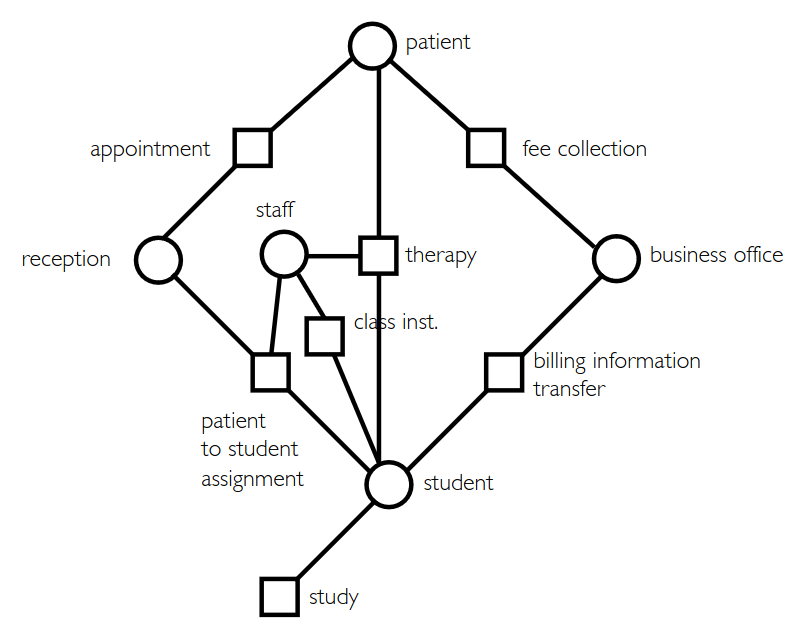
\includegraphics[scale=0.4]{images/UniBoston.png}
    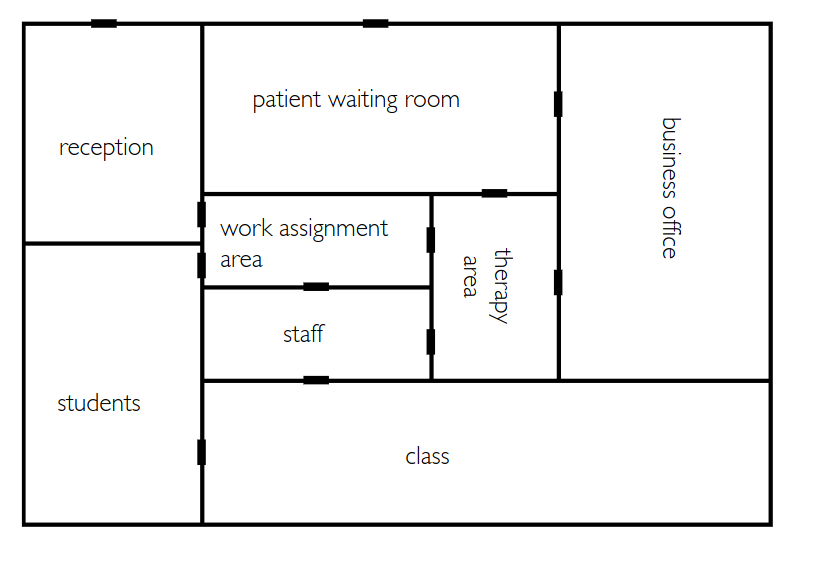
\includegraphics[scale=0.4]{images/UniBoston2.png}
    \caption{Il sistema di classificazione della scuola dentistica dell'Università di Boston.}
\end{figure}

\pagebreak

\begin{figure}
    \centering
    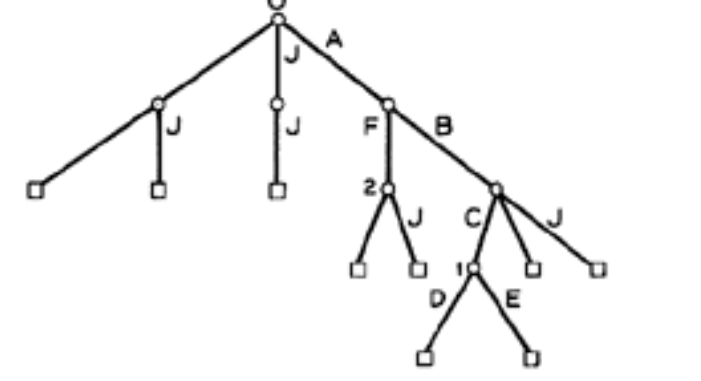
\includegraphics[scale=0.5]{images/Unix.png}
    \caption{Filesystem UNIX.}
\end{figure}

\begin{figure}
    \centering
    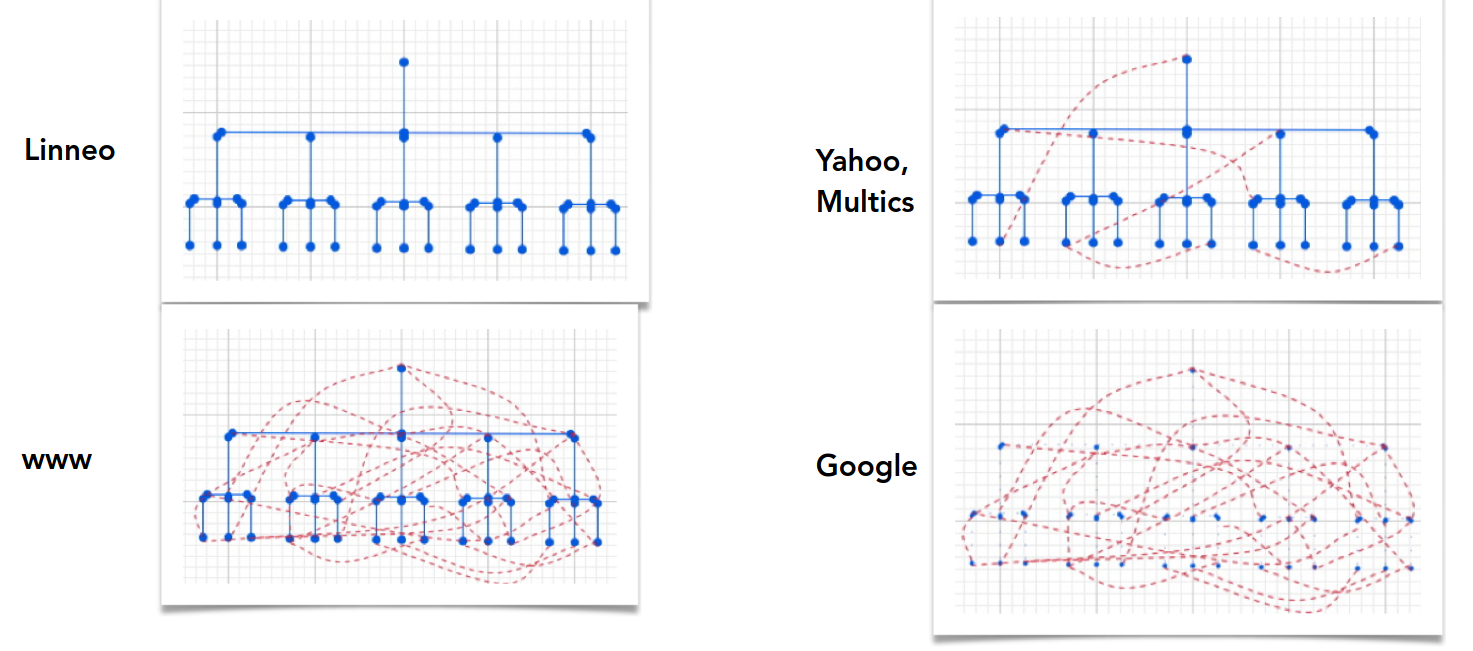
\includegraphics[scale=0.3]{images/C.png}
    \caption{Evoluzione delle gerarchie di classificazione.}
\end{figure}
